%=======================================================================================================================
\section{Jet axis for the one-point correlator}
\label{app:axes}

The one-point correlator (E1C) in the rest frame of the hadronically decaying boson is the energy flow of its decay,
which is sensitive to the parity-even part of its spin-density matrix (Appendix~\ref{app:truth:decay}
and Ref.~\cite[App.~D]{Gao:2026bvp}). The boson direction is not observed, and the frame has to be built from an axis
of the jet. This appendix describes the axes that are implemented, the lab-to-rest-frame conversion, the method used
to compare the axes, and the results so far.

%-----------------------------------------------------------------------------------------------------------------------
\subsection{Strategy: lab-frame tables and the boost offline}
\label{app:axes:strategy}
The boost from the lab to a rest frame along an axis acts on each particle separately and leaves the azimuth $\phi$
about the axis unchanged (Ref.~\cite[App.~D]{Gao:2026bvp}). An unbinned lab-frame E1C about a given axis, together with
that axis and the jet momentum, therefore determines the rest-frame E1C for any boson-mass hypothesis. The expensive
step, recomputing the polar angles about each axis from the constituents, runs in the production (one table per
axis); the boost runs in the analysis, which allows the mass hypothesis and the frame to be changed without
reprocessing.

%-----------------------------------------------------------------------------------------------------------------------
\subsection{Axis definitions}
\label{app:axes:definitions}
\code{EECJetAxisProducer} (\code{JetSetup}) computes each axis of \code{jets.collections.<C>.axes} for the nominal jets,
from all PUPPI-weighted constituents before the constituent selection (i.e.\ including neutral particles), and stores
the four-momentum and a status per axis in the jet table (Section~\ref{sec:axes}). Status 2 means that the axis is not
available; the axis is then the jet four-momentum.
\begin{description}[style=nextline]
\item[\code{jet}] the jet four-momentum after JEC and JER (the existing \code{E1CLab} frame).
\item[\code{axisSoftDrop}] soft drop~\cite{Larkoski:2014wba} with the parameters of the MiniAOD \code{SoftDropPuppi}
  subjets ($\beta = 0$, $z_\mathrm{cut} = 0.1$, $R_0 = 0.8$; the constituents are reclustered with
  Cambridge--Aachen and declustered); the axis is the sum of the two subjets, each corrected with the AK4 PUPPI JEC and,
  in simulation, the AK4 hybrid JER (Section~\ref{sec:axes}). Status 1: grooming ended on a single particle, which
  is then the axis.
\item[\code{axisSoftDropB1}, \code{axisSoftDropZ005}] lighter grooming: $\beta = 1$, $z_\mathrm{cut} = 0.1$; and
  $\beta = 0$, $z_\mathrm{cut} = 0.05$. Uncorrected subjets.
\item[\code{axisTrim}] trimming~\cite{Krohn:2009th}: $k_\mathrm{T}$ subjets of radius $R_\mathrm{sub} = 0.2$, keeping
  those with more than $f_\mathrm{cut} = 3\%$ of the jet $\pt$, the parameters of the CMSSW \code{ak8PFJetsCHSTrimmed}
  configuration; the axis is the sum of the kept subjets, uncorrected.
\item[\code{axisWtaCA}, \code{axisWtaKT}] winner-take-all axis~\cite{Larkoski:2014uqa}: the constituents are reclustered
  into one jet with Cambridge--Aachen or $k_\mathrm{T}$ and the \textsc{FastJet} recombination scheme
  \code{WTA\_pt\_scheme}, in which a merged object takes the rapidity, azimuth and mass of the input with the larger
  $\pt$ and the sum of the two $\pt$ (\textsc{FastJet} 3.4.1, \code{JetDefinition.hh}). This scheme is boost-invariant
  along the beam, consistent with the $(y,\phi)$ clustering metric; \code{WTA\_modp\_scheme} (the direction of the
  larger $|\vec p|$) is not used.
\item[\code{axisRecoil}] the azimuth of the boson of the first passing back-to-back channel (in the order of the
  configuration: \code{Zmumu}, then \code{Zee}) plus $\pi$, and the jet pseudorapidity; status 2 without such a boson.
\item[\code{axisTruth}] in simulation, from \code{prunedGenParticles}, within $\Delta R < 0.8$:
  \begin{itemize}
  \item status 0: the four-momentum of the nearest hadronic boson, a $\gamma$, $Z$, $W$ or $H$ that is the last copy
    in the pruned record (no daughter of the same identity) and has a quark or gluon daughter. A photon must come from
    the hard process, which excludes $\gamma\to q\bar q$ splittings of the QED shower. $H\to WW^*, ZZ^*$ gives the
    $W$/$Z$, not the $H$.
  \item without such a boson, the nearest outgoing hard-process quark or gluon (Pythia~8 status 23, i.e.\ before
    FSR): status 1 if its mother is a boson (a quark of a resolved decay), status 3 otherwise.
  \item status 2: in data, or without a match.
  \end{itemize}
  In the $W$/$Z$ samples the photon and Higgs terms change nothing (the generators label the $\gamma^*/Z$ propagator
  $Z$): on 3000 events each of \code{ZZto2L2Q} and \code{WZto2L2Q} and 3000
  Drell--Yan events, this rule selects exactly the bosons of the previous one (last-copy $W$/$Z$ with a quark or
  gluon daughter), and no photon has a quark or gluon daughter; on 2000 \code{GluGluHto2B\_PT-200} events it selects
  one $H$ per event. In the NANO of one \code{ZZto2L2Q} file (102 events), the status-0 jets and their axes are
  identical to those of the previous rule, and 15 of the 16 previously unmatched reco jets get a parton (status 3);
  all 388 reco jets of 1000 Drell--Yan $\pt^{\ell\ell}$ 400--600\GeV events do. A parton axis has the mass of the
  record (0 for gluons and MadGraph light quarks; 0.33, 0.5 and 4.8\GeV for $u/d$, $s$ and $b$ in the Powheg samples),
  so a rest-frame boost about it needs a fixed mass hypothesis; \code{addRestFrame} rejects only masses below
  $2m_\pi$.
\end{description}
Gen jets get the same axes without corrections. The groomers and the WTA axis are tested with constructed jets
(\code{JetSetup/test/test\_axes.cc}: a soft wide-angle particle groomed away, a single-particle result, an empty jet,
the trimming threshold, the winner of the WTA recombination); deliberately altered versions fail 3 of 7 and 5 of 17
assertions.

%-----------------------------------------------------------------------------------------------------------------------
\subsection{Per-axis lab-frame tables}
\label{app:axes:tables}
For each axis, an unbinned E1C with $\pt$ weights ($n = 1$, normalised to the jet $\pt$) in the \code{jetAxis} frame
about that axis is written for the nominal jets (\code{E1CLab<Axis>}; Section~\ref{sec:eec}). The normalisation still
uses the jet, so the weight of each entry is $\pt^i/\ptj$ for every axis. For jets whose truth axis falls back to the
jet (status 2), \code{E1CLabTruth} equals \code{E1CLab} entry by entry.

%-----------------------------------------------------------------------------------------------------------------------
\subsection{Lab-to-rest-frame conversion}
\label{app:axes:boost}
The conversion is in \code{analysis/bvana/frames.py} and is exposed in the histogram configuration as
\code{restFrame: \{axis, mass\}} (the axis name and either the axis mass or a fixed boson-mass hypothesis). For each
entry $(\theta', \phi)$ of \code{E1CLab<Axis>}, with axis direction $\hat a$, frame axis $\hat x$ (towards the beam on
the side of the axis, orthogonalised) and $\hat y = \hat a\times\hat x$:
\begin{enumerate}
\item The particle direction is $\hat n = \sin\theta'\cos\phi\,\hat x + \sin\theta'\sin\phi\,\hat y + \cos\theta'\,\hat a$,
  its transverse momentum is $\pt^i = w_i\,\ptj$, and $p = \pt^i/|\hat n_\perp|$.
\item Every particle is given the charged-pion mass, at reco and gen level alike, so that the observable is defined
  identically at both levels: $E = (p^2 + m_\pi^2)^{1/2}$. (Reco charged PF candidates carry $m_\pi$; using massless
  particles instead changes the rest-frame angles measurably, which the closure test below detects.)
\item The boost is along $\hat a$, with the axis momentum $P = \pt^\mathrm{axis}\cosh\eta^\mathrm{axis}$ and the mass
  hypothesis $M$: $E_a = (P^2+M^2)^{1/2}$, $\gamma = E_a/M$, $\beta = P/E_a$. The longitudinal rest-frame momentum
  $p^*_\parallel = \gamma(p\cos\theta' - \beta E)$ is computed without cancellation as
  \begin{equation}
    p^*_\parallel = \gamma\left[(1-\beta)E - \frac{m_\pi^2}{E + p} - 2p\sin^2\frac{\theta'}{2}\right],
    \qquad 1 - \beta = \frac{M^2}{E_a(E_a + P)},
  \end{equation}
  which follows from $p\cos\theta' - \beta E = (p - E) + (1-\beta)E - 2p\sin^2(\theta'/2)$ and $E - p = m_\pi^2/(E+p)$.
  Then $p^*_\perp = p\sin\theta'$, $E^* = \gamma(E - \beta p\cos\theta')$, $\theta^* = \operatorname{atan2}(p^*_\perp,
  p^*_\parallel)$ and $\phi^* = \phi$. The rest-frame energy weight is $E^*/M$.
\end{enumerate}
Tests (\code{analysis/tests/test\_frames.py}): a round trip through an explicit Lorentz boost closes to $10^{-9}$; the
massless hypothesis is distinguished from the pion mass; and, on a NANO with constituents, the boost of \code{E1CLab}
about the jet with the jet mass is compared entry by entry with the C++ \code{E1CHelicity}, which boosts the stored
four-vectors. For unit-PUPPI-weight pions with stored mass $m_\pi$ and $p^* > 0.5\GeV$ the 99\% quantile of
$|\Delta\theta^*|$ is below $10^{-4}$ (maximum $1.1\times10^{-4}$) and $|\Delta\phi^*| < 10^{-5}$. The comparison is
restricted to these particles because the C++ scales the whole four-vector by the PUPPI weight (mass $w\,m_\pi$), and
for $p^* \to 0$ the rest-frame direction is undefined (such particles have small weights).

%-----------------------------------------------------------------------------------------------------------------------
\subsection{Comparison method}
\label{app:axes:method}
\code{analysis/axisStudy.py} uses reco or gen jets of the signal samples \code{ZZto2L2Q} and \code{WZto2L2Q} that are
matched to a truth boson (\code{axisTruthStatus} 0) whose mass lies in the window of the truth definition
(Appendix~\ref{app:truth}: $66$--$116\GeV$ for the $Z$, $60$--$100\GeV$ for the $W$), and to an LHE hadronic boson within
$\Delta R < 0.4$. The jet weight $w_j$ is the generator weight, times the reweighting factor below where it applies. For
each axis:
\begin{itemize}
\item the distance $\Delta R$ between the axis and the truth boson (Section~\ref{app:axes:dr});
\item the rest-frame E1C with the truth boson mass as $M$, so that only the axis differs, weighted by the rest-frame
  energy $E^*/M$; its moments $\langle P_2(\cos\theta^*)\rangle$, $\langle\sin^2\theta^*\cos2\phi^*\rangle$,
  $\langle\sin2\theta^*\cos\phi^*\rangle$ and $\langle\cos\theta^*\rangle$, computed as ratios of sums over jets
  ($R = \sum_j w_j N_j / \sum_j w_j D_j$, with $N_j = \sum_{i\in j} e_i g(\theta_i,\phi_i)$ and $D_j = \sum_{i\in j} e_i$),
  with delta-method uncertainties from the per-jet influence $w_j(N_j - R D_j)/\sum w D$, which keeps the correlations
  of the entries of a jet;
\item the same moments with the jets reweighted to pure longitudinal or pure transverse bosons
  (Appendix~\ref{app:truth:reweighting}), with the truth $\rho_{00}$ of the unselected LHE sample in the LHE boson $\pt$
  bin. The \emph{sensitivity} $S = \langle P_2\rangle_T - \langle P_2\rangle_L$ is the response of the observable to
  $\rho_{00}$; an axis that degrades the information on the boson direction reduces $S$.
\end{itemize}
All axes are evaluated on the same jets, so the difference of the sensitivities of two axes has an uncertainty from
the difference of their per-jet influences, which includes their (large) correlation.

%-----------------------------------------------------------------------------------------------------------------------
\subsection{Distance to the truth boson}
\label{app:axes:dr}
Figures~\ref{fig:dr} and~\ref{fig:drmedian} and Table~\ref{tab:dr} show the distance $\Delta R$ (pseudorapidity and
azimuth) between each axis and the truth boson (\code{analysis/axisDeltaR.py}), for jets matched to a truth boson whose
mass lies between 60 and 116\GeV{} (the union of the $W$ and $Z$ windows of Appendix~\ref{app:truth}); without this
requirement, low-mass $\gamma^*\to q\bar q$ ``bosons'' of the \code{ZZto2L2Q} sample, generated down to $4\GeV$, enter.
The sample is 23 files of \code{ZZto2L2Q} (15) and \code{WZto2L2Q} (8), processed with the configuration of this note;
one further \code{ZZto2L2Q} file (707 events) has no selected event. This gives 1743 reco and 1876 gen jets, weighted with
the generator weight.
\begin{itemize}
\item The jet axis is the closest to the boson at every $\pt$: median $\Delta R$ 0.059, 0.027, 0.017 and 0.009 for reco
  jets with $\pt$ 200--300, 300--400, 400--600 and above $600\GeV$. The groomed and trimmed axes are slightly farther
  (by up to 0.006 in the median); not studied further.
\item The winner-take-all axes follow the harder of the two quarks, not the boson: their median distance is 0.18 at
  200--300\GeV{} and falls with $\pt$ like the opening angle of the decay (Eq.~\eqref{eq:app:containment}). The
  Cambridge--Aachen and $k_\mathrm{T}$ versions are indistinguishable.
\item The recoil axis is at a median 0.07--0.10; its azimuth is that of the dilepton system, which also recoils against
  additional radiation (not verified separately).
\item All axes have a tail: 10\% of the jets lie beyond $\Delta R \approx 0.2$ from the boson even for the jet axis.
  At 200--300\GeV, 5\% lie beyond 0.44; jets containing only one of the quarks (Appendix~\ref{app:truth:bias}) are a
  likely source, which has not been checked jet by jet.
\item Soft drop ends on a single particle (status 1) for at most 0.8\% of the jets, and no axis is unavailable
  (status 2) for these truth-matched jets.
\end{itemize}

\begin{figure}[htbp]
\centering
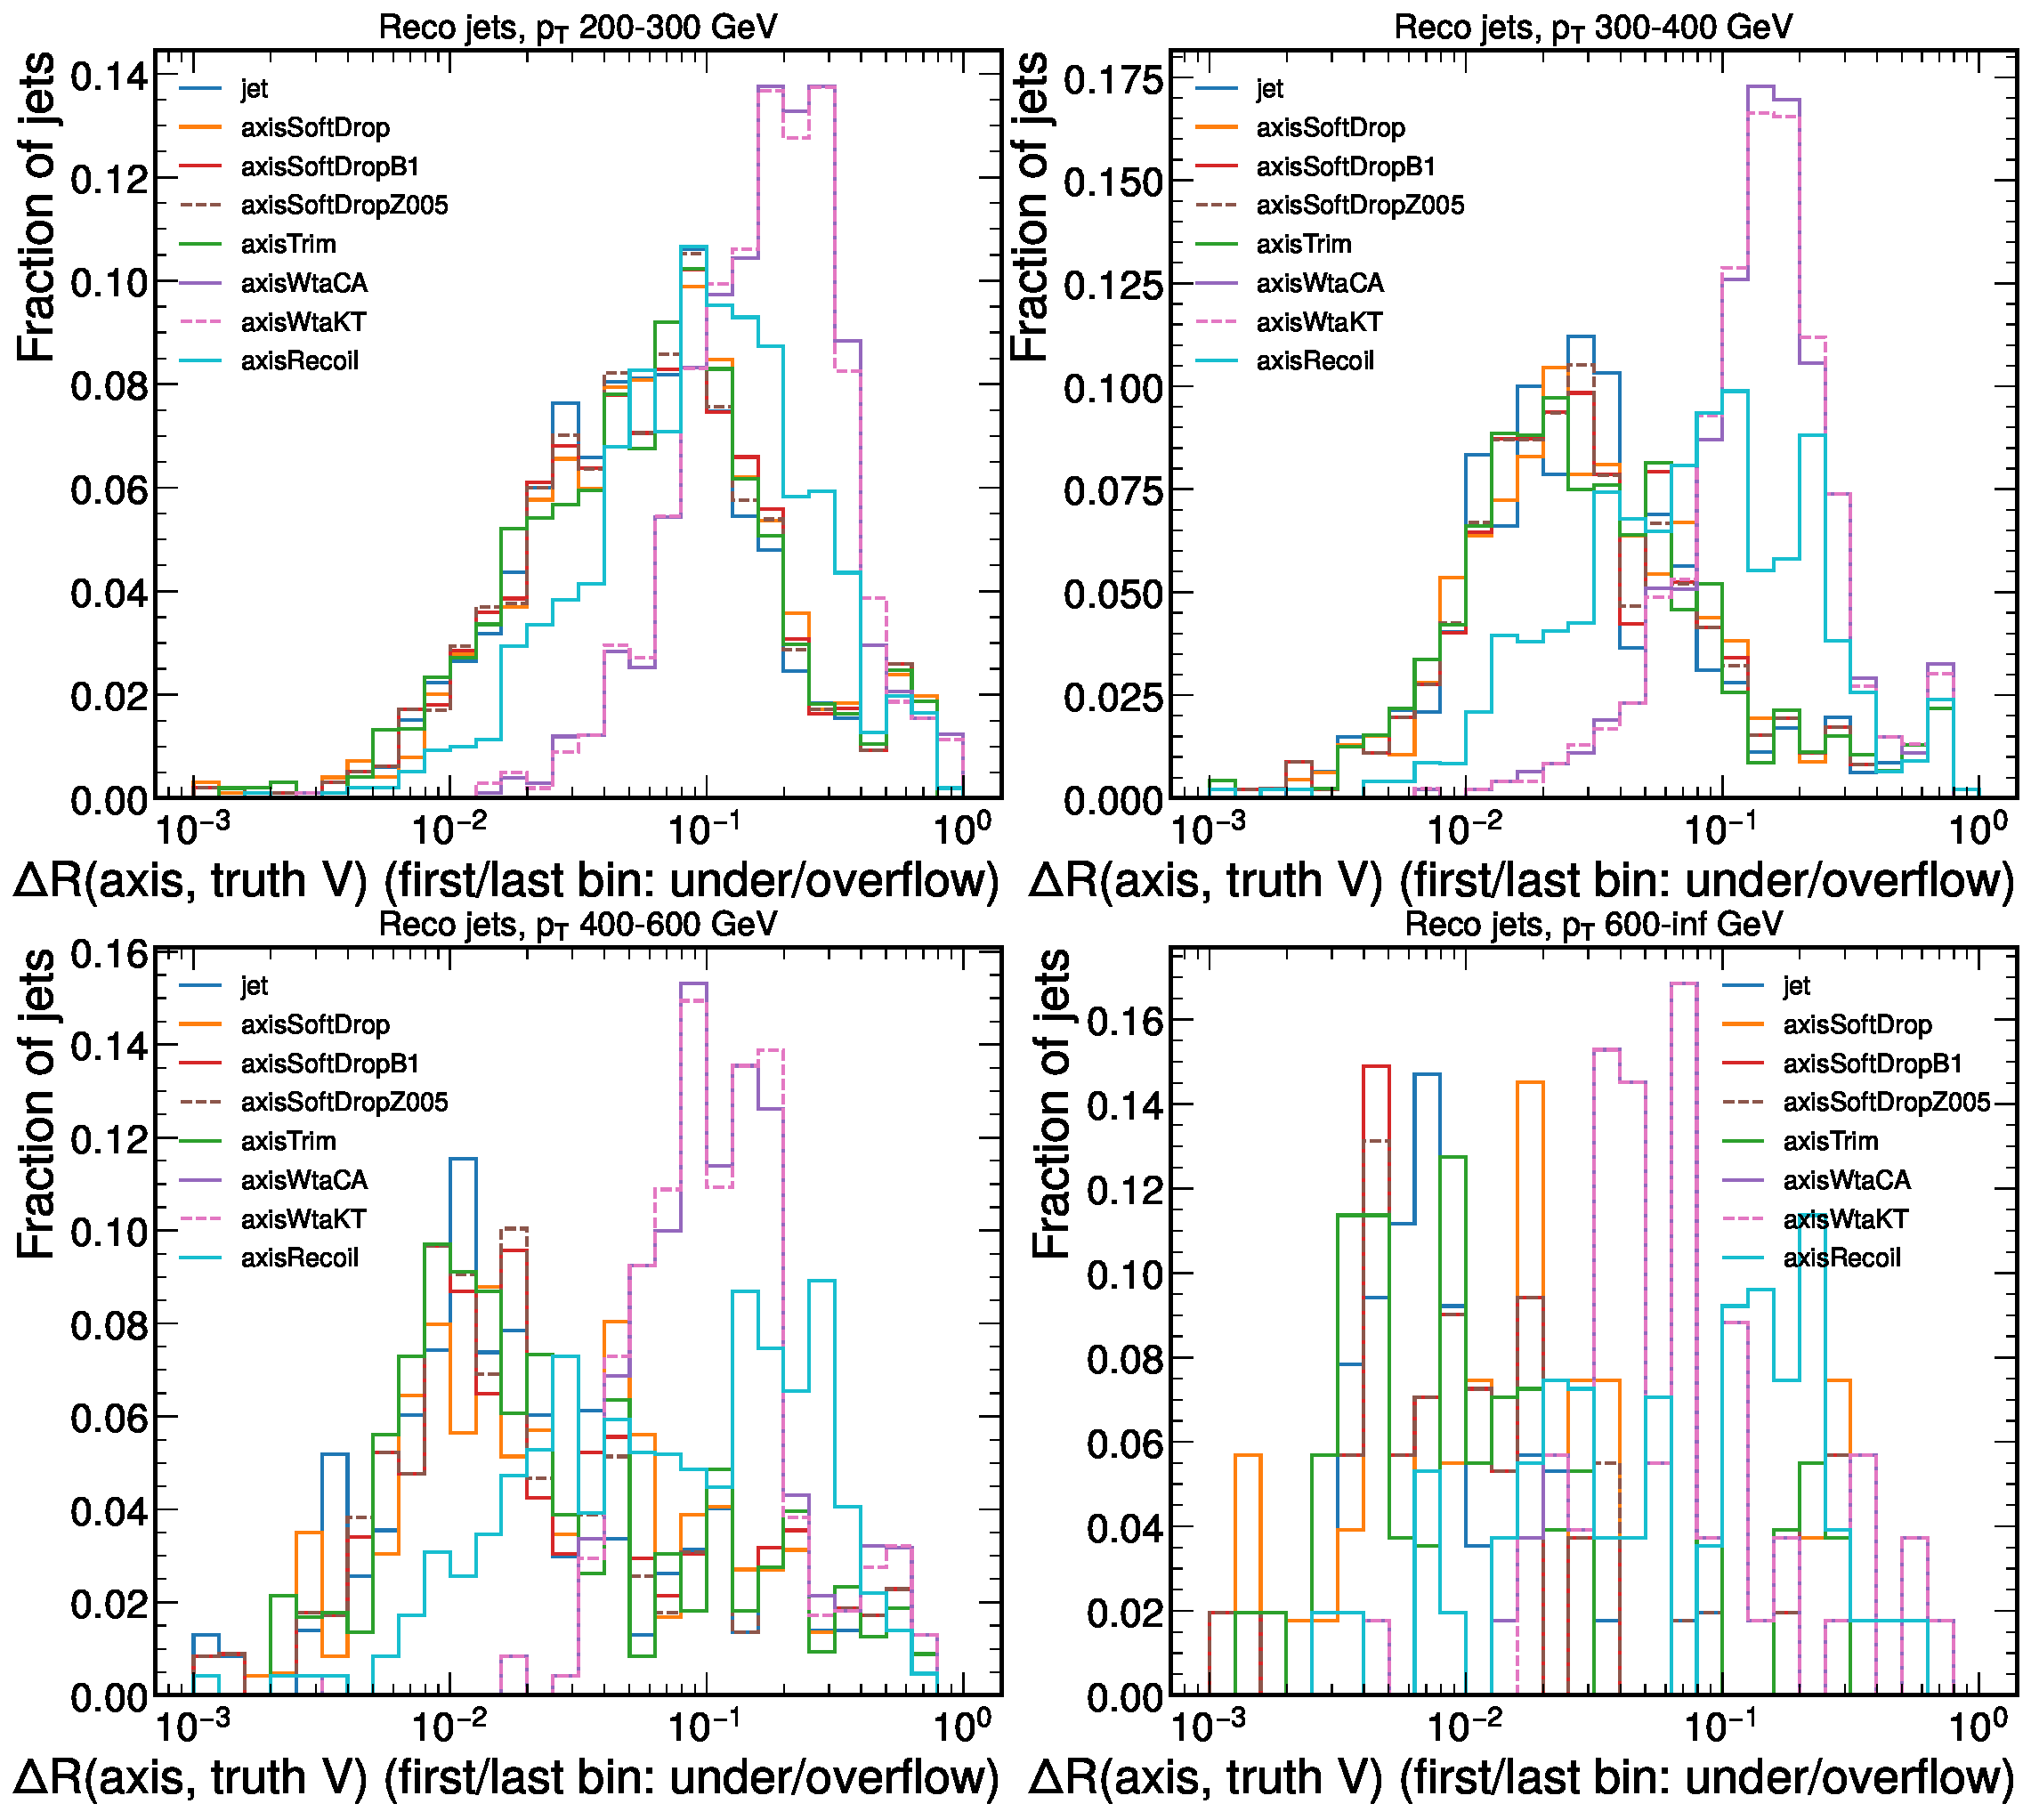
\includegraphics[width=0.49\textwidth]{figures/dR_Reco.pdf}\hfill
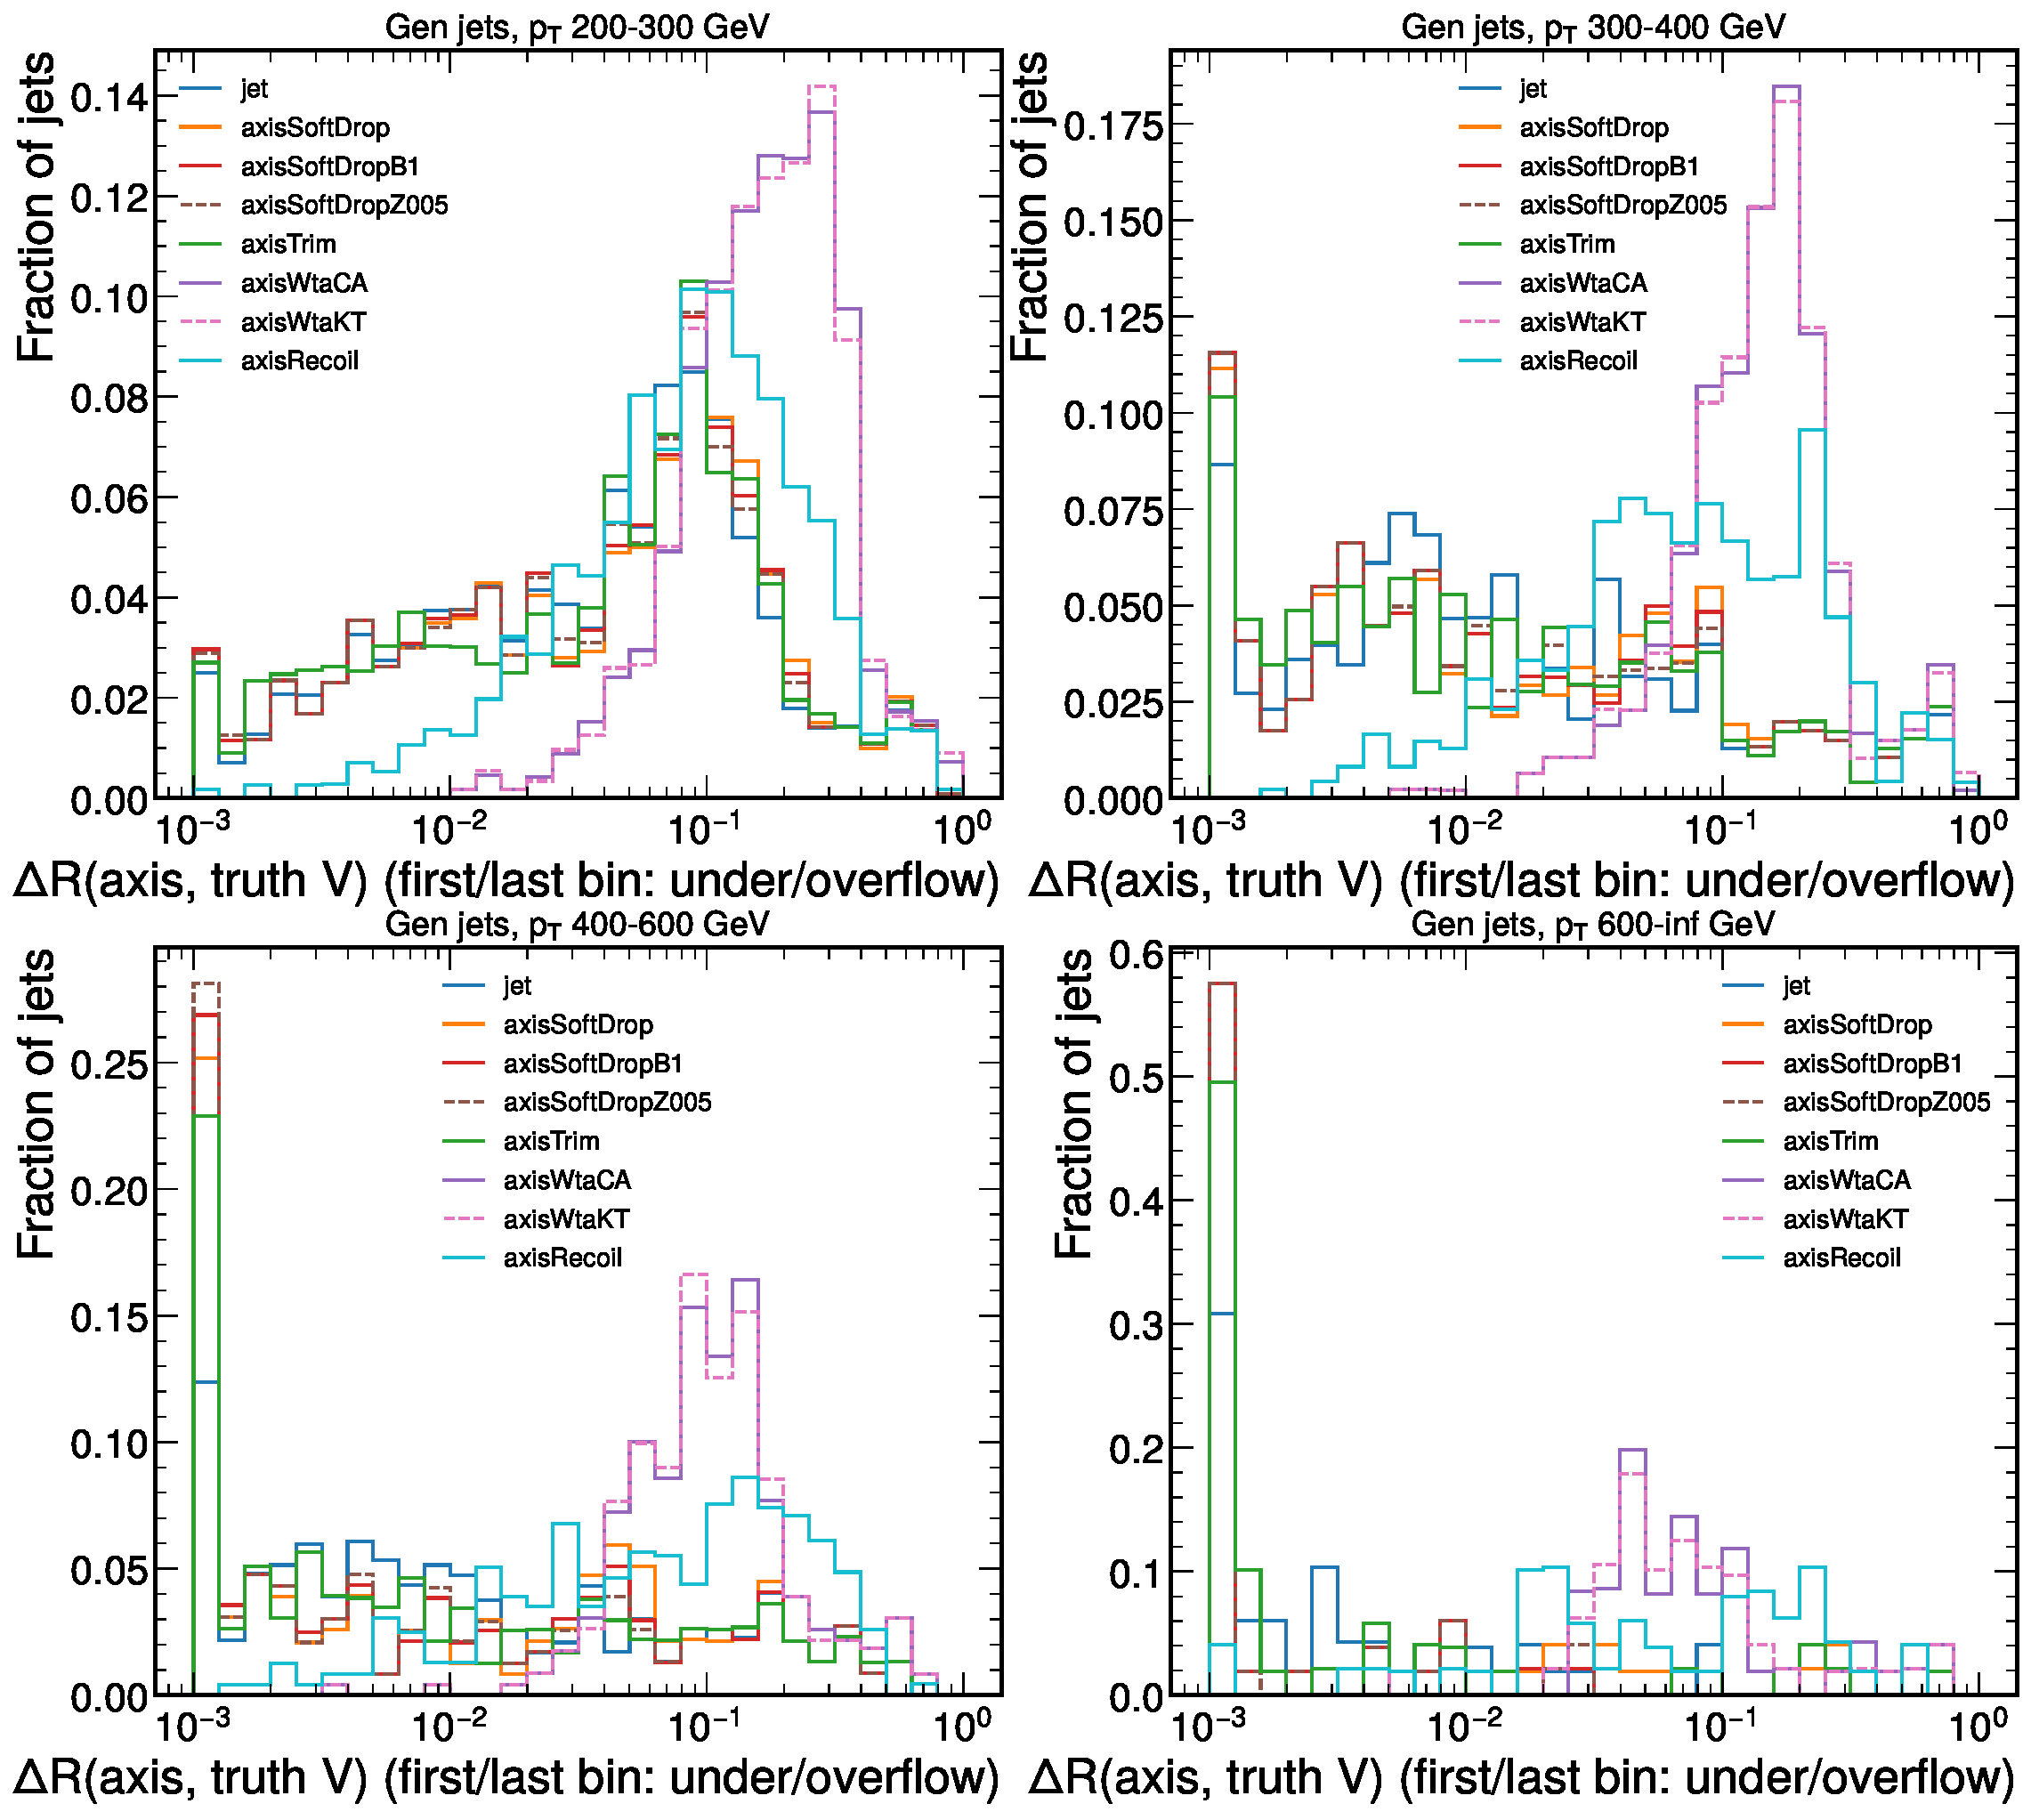
\includegraphics[width=0.49\textwidth]{figures/dR_Gen.pdf}
\caption{Distribution of $\Delta R$ between each axis and the truth boson, normalised to the number of jets, in four bins
of jet $\pt$ (200--300, 300--400, 400--600 and above $600\GeV$), for reco jets (left) and gen jets (right). Logarithmic
bins between $10^{-3}$ and 1; the first and last bins contain the under- and overflow.}
\label{fig:dr}
\end{figure}

\begin{figure}[htbp]
\centering
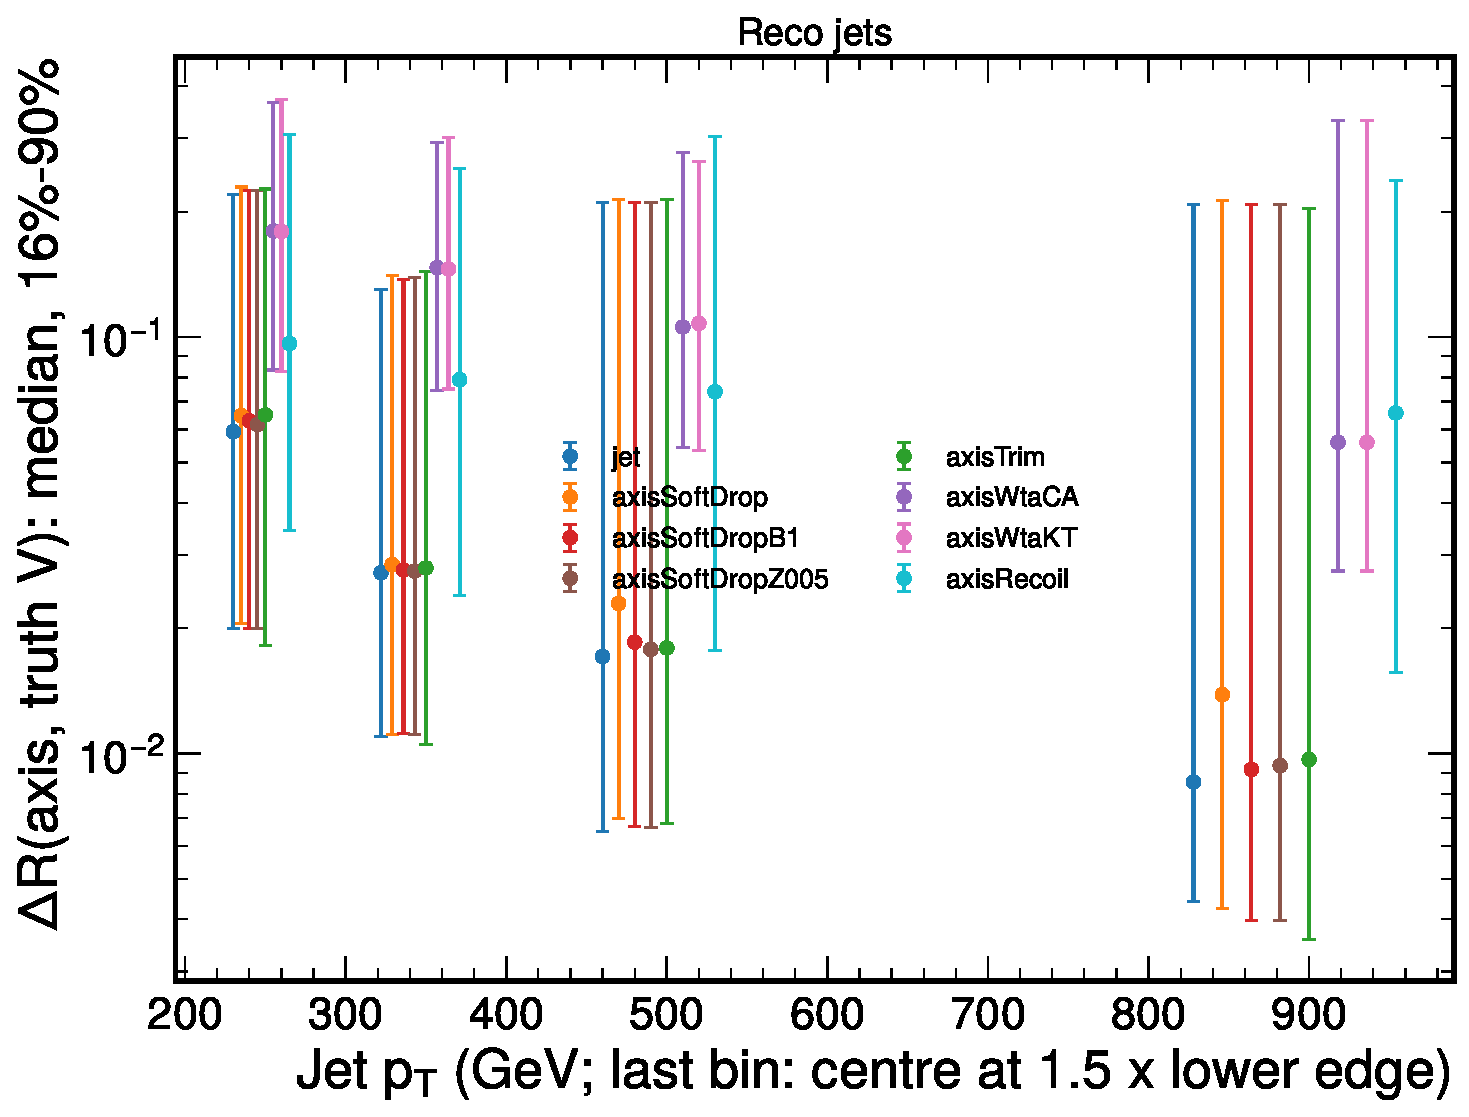
\includegraphics[width=0.49\textwidth]{figures/dRmedian_Reco.pdf}\hfill
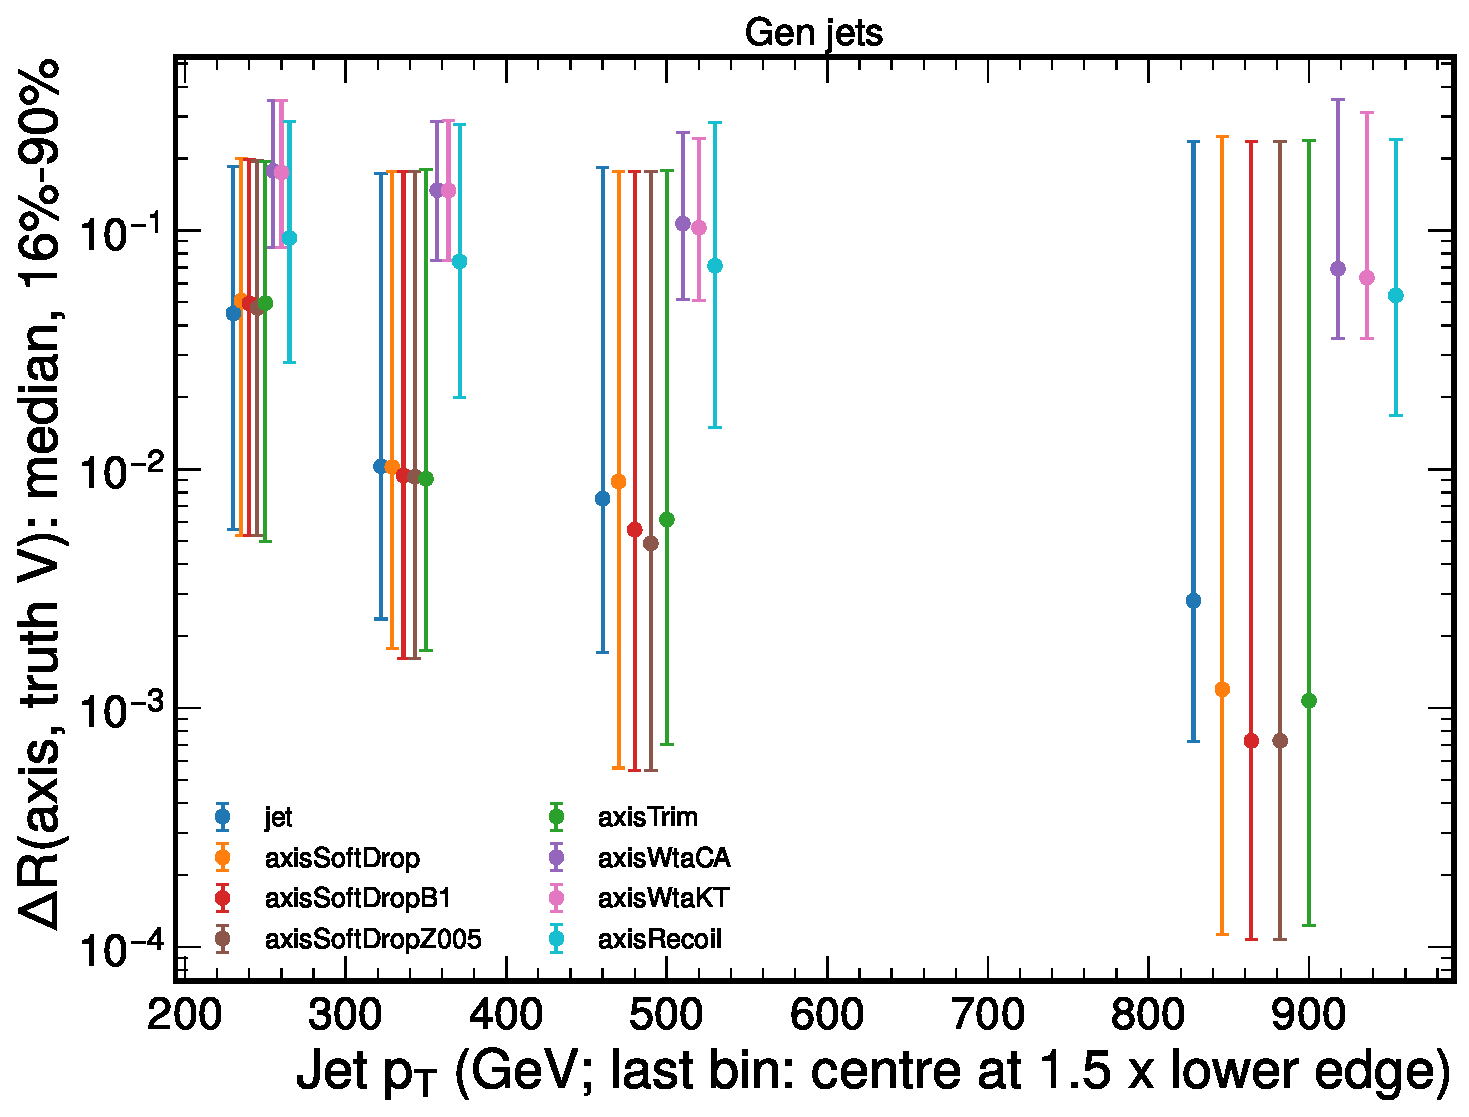
\includegraphics[width=0.49\textwidth]{figures/dRmedian_Gen.pdf}
\caption{Median of $\Delta R$ between each axis and the truth boson versus jet $\pt$ (markers), with the interval
between the 16\% and 90\% quantiles (bars); reco jets (left) and gen jets (right). The markers of each $\pt$ bin are
displaced horizontally for readability.}
\label{fig:drmedian}
\end{figure}

\begin{table}[htbp]
\centering
\caption{Median and 90\% quantile of $\Delta R$(axis, truth boson), and the fraction of jets with $\Delta R < 0.05$, per
bin of jet $\pt$. Reco jets: 990, 470, 229 and 54 jets per bin; gen jets: 1124, 472, 231 and 49. The full tables, with
the mean and the 68\% and 95\% quantiles, are in \code{dR.md} of the study directory.}
\label{tab:dr}
\footnotesize
\setlength{\tabcolsep}{3pt}
\begin{tabular}{lcccccccccccc}
\toprule
 & \multicolumn{3}{c}{200--300\GeV} & \multicolumn{3}{c}{300--400\GeV} & \multicolumn{3}{c}{400--600\GeV} & \multicolumn{3}{c}{$> 600\GeV$} \\
axis & q50 & q90 & $f_{<0.05}$ & q50 & q90 & $f_{<0.05}$ & q50 & q90 & $f_{<0.05}$ & q50 & q90 & $f_{<0.05}$ \\
\midrule
\multicolumn{13}{l}{\emph{reco jets}} \\
jet & 0.059 & 0.22 & 0.44 & 0.027 & 0.13 & 0.71 & 0.017 & 0.21 & 0.74 & 0.009 & 0.21 & 0.81 \\
soft drop & 0.065 & 0.23 & 0.41 & 0.028 & 0.14 & 0.68 & 0.023 & 0.21 & 0.68 & 0.014 & 0.21 & 0.81 \\
soft drop $\beta=1$ & 0.063 & 0.22 & 0.43 & 0.028 & 0.14 & 0.68 & 0.018 & 0.21 & 0.72 & 0.009 & 0.21 & 0.81 \\
soft drop $z_\mathrm{cut}=0.05$ & 0.062 & 0.23 & 0.43 & 0.027 & 0.14 & 0.69 & 0.018 & 0.21 & 0.73 & 0.009 & 0.21 & 0.81 \\
trimming & 0.065 & 0.23 & 0.42 & 0.028 & 0.14 & 0.69 & 0.018 & 0.21 & 0.74 & 0.010 & 0.20 & 0.81 \\
WTA C/A & 0.180 & 0.37 & 0.06 & 0.147 & 0.29 & 0.08 & 0.106 & 0.28 & 0.12 & 0.056 & 0.33 & 0.45 \\
WTA $k_\mathrm{T}$ & 0.179 & 0.37 & 0.06 & 0.146 & 0.30 & 0.07 & 0.108 & 0.26 & 0.12 & 0.056 & 0.33 & 0.45 \\
recoil & 0.097 & 0.31 & 0.25 & 0.079 & 0.25 & 0.35 & 0.074 & 0.30 & 0.41 & 0.066 & 0.24 & 0.42 \\
\midrule
\multicolumn{13}{l}{\emph{gen jets}} \\
jet & 0.045 & 0.18 & 0.52 & 0.010 & 0.17 & 0.77 & 0.007 & 0.18 & 0.76 & 0.003 & 0.24 & 0.81 \\
soft drop & 0.051 & 0.20 & 0.50 & 0.010 & 0.18 & 0.72 & 0.009 & 0.18 & 0.73 & 0.001 & 0.25 & 0.80 \\
soft drop $\beta=1$ & 0.050 & 0.20 & 0.50 & 0.009 & 0.18 & 0.72 & 0.006 & 0.18 & 0.76 & 0.001 & 0.24 & 0.81 \\
soft drop $z_\mathrm{cut}=0.05$ & 0.047 & 0.20 & 0.51 & 0.009 & 0.18 & 0.75 & 0.005 & 0.18 & 0.76 & 0.001 & 0.24 & 0.81 \\
trimming & 0.050 & 0.19 & 0.51 & 0.009 & 0.18 & 0.75 & 0.006 & 0.18 & 0.76 & 0.001 & 0.24 & 0.81 \\
WTA C/A & 0.178 & 0.35 & 0.06 & 0.147 & 0.29 & 0.08 & 0.107 & 0.26 & 0.14 & 0.069 & 0.35 & 0.37 \\
WTA $k_\mathrm{T}$ & 0.175 & 0.35 & 0.06 & 0.147 & 0.29 & 0.08 & 0.102 & 0.24 & 0.14 & 0.063 & 0.31 & 0.37 \\
recoil & 0.093 & 0.28 & 0.28 & 0.074 & 0.28 & 0.38 & 0.071 & 0.28 & 0.40 & 0.053 & 0.24 & 0.49 \\
\bottomrule
\end{tabular}
\end{table}


%-----------------------------------------------------------------------------------------------------------------------
\subsection{Sensitivity to $\rho_{00}$}
\label{app:axes:results}
The sensitivity is evaluated on jets matched to a truth boson in its mass window (Appendix~\ref{app:truth}) and to an
LHE hadronic boson within $\Delta R < 0.4$, for which the truth $\rho_{00}$ of the unselected samples
(\code{rho\_ZZ.json} and \code{rho\_WZ.json}, hadronic decays) is available: 1728 reco and 1859 gen jets of the same 23
files. The mass window matters: without it, three jets matched to $\gamma^*\to q\bar q$ of 4--6\GeV, boosted with
$\gamma \approx 100$, carried 42\% of the total rest-frame energy weight and inflated the uncertainties of all axes but
the truth one by more than an order of magnitude (a first version of the study, quoted in earlier notes, suffered from this).

\begin{table}[htbp]
\centering
\caption{Rest-frame-energy-weighted E1C moments about each axis (boost with the truth boson mass): the nominal
$\langle P_2(\cos\theta^*)\rangle$, its values after reweighting to pure longitudinal ($L$) and pure transverse ($T$)
bosons, and the sensitivity $S = \langle P_2\rangle_T - \langle P_2\rangle_L$, with the paired differences of $S$ with
respect to the jet axis and to the truth axis (uncertainties include the correlation of the axes, which share the jets).
Also the nominal $\langle\sin^2\theta^*\cos2\phi^*\rangle$.}
\label{tab:axisresults}
\scriptsize
\setlength{\tabcolsep}{2.5pt}
\begin{tabular}{lccccccc}
\toprule
axis & $\langle P_2\rangle$ & $\langle P_2\rangle_L$ & $\langle P_2\rangle_T$ & $S$ & $S - S_\mathrm{jet}$ & $S - S_\mathrm{truth}$ & $\langle\sin^2\theta^*\cos2\phi^*\rangle$ \\
\midrule
\multicolumn{8}{l}{\emph{reco jets (1728)}} \\
jet & $0.076 \pm 0.009$ & $-0.064$ & $0.093$ & $0.157 \pm 0.006$ & --- & $+0.008 \pm 0.005$ & $-0.007$ \\
soft drop & $0.105 \pm 0.010$ & $-0.047$ & $0.122$ & $0.169 \pm 0.007$ & $+0.013 \pm 0.001$ & $+0.021 \pm 0.005$ & $-0.007$ \\
soft drop $\beta = 1$ & $0.091 \pm 0.010$ & $-0.061$ & $0.109$ & $0.170 \pm 0.006$ & $+0.013 \pm 0.001$ & $+0.021 \pm 0.005$ & $-0.007$ \\
soft drop $z_\mathrm{cut} = 0.05$ & $0.092 \pm 0.010$ & $-0.062$ & $0.109$ & $0.171 \pm 0.006$ & $+0.014 \pm 0.001$ & $+0.022 \pm 0.005$ & $-0.007$ \\
trimming & $0.091 \pm 0.009$ & $-0.060$ & $0.109$ & $0.168 \pm 0.006$ & $+0.012 \pm 0.001$ & $+0.020 \pm 0.005$ & $-0.007$ \\
WTA C/A & $0.365 \pm 0.007$ & $0.286$ & $0.374$ & $0.088 \pm 0.005$ & $-0.069 \pm 0.004$ & $-0.060 \pm 0.005$ & $0.020$ \\
WTA $k_\mathrm{T}$ & $0.363 \pm 0.008$ & $0.283$ & $0.373$ & $0.090 \pm 0.005$ & $-0.067 \pm 0.004$ & $-0.059 \pm 0.006$ & $0.020$ \\
recoil & $0.024 \pm 0.009$ & $-0.061$ & $0.035$ & $0.095 \pm 0.006$ & $-0.061 \pm 0.005$ & $-0.053 \pm 0.007$ & $-0.129$ \\
truth & $0.000 \pm 0.009$ & $-0.132$ & $0.017$ & $0.149 \pm 0.007$ & $-0.008 \pm 0.005$ & --- & $-0.008$ \\
\midrule
\multicolumn{8}{l}{\emph{gen jets (1859)}} \\
jet & $0.074 \pm 0.009$ & $-0.081$ & $0.093$ & $0.173 \pm 0.006$ & --- & $+0.015 \pm 0.005$ & $-0.005$ \\
soft drop & $0.100 \pm 0.010$ & $-0.068$ & $0.119$ & $0.187 \pm 0.007$ & $+0.014 \pm 0.001$ & $+0.029 \pm 0.005$ & $-0.004$ \\
soft drop $\beta = 1$ & $0.084 \pm 0.009$ & $-0.076$ & $0.103$ & $0.179 \pm 0.006$ & $+0.006 \pm 0.001$ & $+0.021 \pm 0.005$ & $-0.005$ \\
soft drop $z_\mathrm{cut} = 0.05$ & $0.084 \pm 0.009$ & $-0.077$ & $0.102$ & $0.179 \pm 0.006$ & $+0.006 \pm 0.0004$ & $+0.021 \pm 0.005$ & $-0.004$ \\
trimming & $0.081 \pm 0.009$ & $-0.078$ & $0.100$ & $0.178 \pm 0.006$ & $+0.005 \pm 0.001$ & $+0.020 \pm 0.005$ & $-0.004$ \\
WTA C/A & $0.398 \pm 0.007$ & $0.321$ & $0.408$ & $0.087 \pm 0.005$ & $-0.086 \pm 0.004$ & $-0.071 \pm 0.006$ & $0.025$ \\
WTA $k_\mathrm{T}$ & $0.396 \pm 0.007$ & $0.318$ & $0.406$ & $0.088 \pm 0.005$ & $-0.085 \pm 0.004$ & $-0.070 \pm 0.006$ & $0.025$ \\
recoil & $0.019 \pm 0.009$ & $-0.076$ & $0.031$ & $0.107 \pm 0.006$ & $-0.066 \pm 0.005$ & $-0.051 \pm 0.006$ & $-0.125$ \\
truth & $0.013 \pm 0.009$ & $-0.127$ & $0.031$ & $0.158 \pm 0.007$ & $-0.015 \pm 0.005$ & --- & $-0.010$ \\
\bottomrule
\end{tabular}
\end{table}

Table~\ref{tab:axisresults} gives the results.
\begin{itemize}
\item The winner-take-all and recoil axes lose 32--45\% of the sensitivity of the truth axis (reco: $-0.060 \pm 0.005$
  and $-0.053 \pm 0.007$, i.e.\ 11 and 8 standard deviations). Their nominal moments are also shifted: WTA raises
  $\langle P_2\rangle$ to 0.36 (an axis along one quark makes the energy flow look aligned with it), and the recoil axis
  produces a spurious $\langle\sin^2\theta^*\cos2\phi^*\rangle = -0.13$, presumably because its error is mostly in
  azimuth. These axes are not suitable.
\item The jet, soft-drop and trimmed axes give a sensitivity equal to or slightly \emph{larger} than that of the truth
  axis (reco: $+0.008$ to $+0.022 \pm 0.005$); the groomed and trimmed axes exceed the jet axis by $0.012$--$0.014$
  with an uncertainty of 0.001 (reco). Their nominal moments differ from those of the truth axis ($\langle P_2\rangle$
  0.08--0.10 against 0.00).
\item A sensitivity above that of the truth axis cannot come from a better knowledge of the boson direction. A
  plausible cause is that these axes are computed from the same particles whose energy flow is measured, so that the
  axis correlates with the decay configuration; this has not been demonstrated. Sensitivity alone therefore does not
  decide between these axes: the bias of the moments with respect to the truth axis, its dependence on $\rho_{00}$, and
  the experimental robustness (pileup, the soft-drop corrections and their uncertainties) also enter.
\end{itemize}
The comparison of 17 November on 24 different files (2127 reco jets) had reached the same qualitative conclusions, with
the larger uncertainties caused by the missing mass window. Open points: a choice among the jet, soft-drop and trimmed
axes; the response matrix of the moments to $\rho_{00}$ including the other density-matrix elements; the restriction to
$\pt \gtrsim 300\GeV$ suggested by Appendix~\ref{app:truth:bias}; and larger samples, especially above $400\GeV$.

